\documentclass{letter}
\usepackage{enumitem}
\usepackage{amsmath}
\usepackage{booktabs}
\usepackage{graphicx}
\usepackage[letterpaper,top=0.1cm,bottom=0.2cm,left=0.2cm,right=0.2cm,marginparwidth=0cm]{geometry}

\newcommand{\textib}[1]{\textit{\textbf{{#1}}}}

\begin{document}
A: Assets, D: Debt, E: Equity, NWC: Net Working Capital, R: Revenue \\
\textib{Basics} \\
Assets = Debt(Liabilities) + Equity \leaders\hbox{$\cdot$}\hfill $\iff$ A = D + E \\
Income = Revenue - Expenses \\
Net Working Capital = (Current Assets) - (Current Liabilities) \leaders\hbox{$\cdot$}\hfill $\iff$ NWC = CA - CL \\
CashFlow(Assets) = CashFlow(Creditors) + CashFlow(Stockholders) \leaders\hbox{$\cdot$}\hfill $\iff$ CF(A) = CF(B) + CF(S) \\
Operating Cashflow = (Net Income) + Depreciation + ($\Delta$NWC) \leaders\hbox{$\cdot$}\hfill $\iff$ OCF = EBIT + Depreciation - Taxes
\newline
\textib{Liquidity Ratios} \\
Current Ratio = (Current Assets)/(Current Liabilities) \leaders\hbox{$\cdot$}\hfill $\iff$ CR = CA/CL \\
Quick Ratio = (Current Assets - Inventory)/(Current Liabilities) \leaders\hbox{$\cdot$}\hfill $\iff$ CR = (CA - Inv)/CL \\
Cash Ratio = Cash/(Current Liabilities) \leaders\hbox{$\cdot$}\hfill $\iff$ Cash/CL
\newline
\textib{Leverage Ratios} \\
Total Debt Ratio = (Assets - Equity)/Assets \leaders\hbox{$\cdot$}\hfill $\iff$ TDR = (A - E)/A \\
Debt/Equity Ratio = Debt/Equity \leaders\hbox{$\cdot$}\hfill $\iff$ D/E \\
Equity Mulitplier = Assets/Equity $\iff$ 1 + Debt/Equity \leaders\hbox{$\cdot$}\hfill $\iff$ EM = A/E $\iff$ 1 + D/E
\newline
\textib{Coverage Ratios} \\
Times Interest Earned = (Earnings Before Interest and Taxes)/Interst \leaders\hbox{$\cdot$}\hfill $\iff$ TIE = EBIT/Interest \\
Cash Coverage = (EBIT + Depreciation + Amortization)/Interest
\newline
\textib{Ratio Analysis} \\
Inventory Turnover = Cost of Goods Sold/Inventory \leaders\hbox{$\cdot$}\hfill $\iff$ IT = COGS/Inventory \\
Days' Sales in Inventory = 365/(Inventory Turnover) \leaders\hbox{$\cdot$}\hfill $\iff$ DSI = 365/IT
\newline
\textib{Receivables Ratios} \\
Receivables Turnover = Sales/(Accounts Receivable) \leaders\hbox{$\cdot$}\hfill $\iff$ RT = S/AR \\
Days' Sales in Receivables = 365/(Receivables Turnover) \leaders\hbox{$\cdot$}\hfill $\iff$ DSR = 365/RT \\
Total Asset Turnover = Sales/(Total Assets) \leaders\hbox{$\cdot$}\hfill $\iff$ TAT = S/A
\newline
\textib{Profitability Ratios} \\
Profit Margin = (Net Income)/Sales \leaders\hbox{$\cdot$}\hfill $\iff$ PM = NI/S \\
Return on Assets = (Net Income)/(Total Assets) \leaders\hbox{$\cdot$}\hfill $\iff$ ROA = NI/A \\
Return on Equity = (Net Income)/(Total Equity) \leaders\hbox{$\cdot$}\hfill $\iff$ ROE = NI/E
\newline
\textib{Market Value Measures} \\
Earnings Per Share = (Net Income)/(Shares Outstanding) \leaders\hbox{$\cdot$}\hfill $\iff$ EPS = NI/SO \\
Price-to-Earnings Ratio = (Price per Share)/(Earnings per Share) \leaders\hbox{$\cdot$}\hfill $\iff$ PE Ratio = PPS/EPS \\
Market Capitalization = (PPS)$\cdot$(Shares Outstanding)
\newline
\textib{Dividend Ratios} \\
Dividend Payout Ratio = (Dividends Paid)/Net Income = $d$ \\
Retention Ratio = 1 - (Dividends Paid)/Net Income \leaders\hbox{$\cdot$}\hfill $\iff$ $b = 1 - d$
\newline
\textib{Du-Pont Identity} \\
ROE = $\frac{NI}{S} \cdot \frac{S}{A} \cdot \frac{A}{E}$ PM$\cdot$TAT$\cdot$EM
\newline
\textib{Pro Forma Income Statement for year $n$} \\
(Projected) Sales$_n$ = Sales$_{n - 1} \cdot$(1 + Growth Rate) \\
(Projected) (Cost of Goods Sold)$_n$ = (Cost of Goods Sold)$_{n - 1} \cdot$(1 + Growth Rate) \\
(Projected) (Taxable Income)$_n$ = Sales$_n$ - Costs$_n$ - Interest$_n$ \\
(Projected) Interest$_n$ = Interest$_{n - 1}$ + (Interest Rate)$\cdot$D \\
(Projected) Taxes$_n$ = (Tax Rate)$\cdot$(Taxable Income)$_n$ \\
(Projected) (Net Income)$_n$ = (Taxable Income$_n$) - Taxes$_n$ \\
(Projected) Dividends$_n$ = (Net Income)$_n \cdot$(Dividend Payout Ratio) \\
(Projected) (Addition to Retained Earnings)$_n$ = (Net Income$_n$) - Dividends$_n$ = ($\Delta$Retained Earnings)
\newline
\textib{Pro Forma Balance Sheet for year $n$} \\
(Projected) Cash$_n$ = Cash$_{n - 1} \cdot$(1 + Growth Rate) \\
(Projected) (Accounts Receivable)$_n$ = (Accounts Receivable)$_{n - 1} \cdot$(1 + Growth Rate) \\
(Projected) Inventory$_n$ = Inventory$_{n - 1} \cdot$(1 + Growth Rate) \\
(Projected) (Net Fixed Assets)$_n$ = (Net Fixed Assets)$_{n - 1} \cdot$(1 + Growth Rate) \\
(Projected) (Accounts Payable)$_n$ = (Accounts Payable)$_{n - 1} \cdot$(1 + Growth Rate) \\
(Projected) (Notes Payable)$_n$ = (Notes Payable)$_{n - 1}$ + D \\
(Projected) (Long Term Debt)$_n$ = (Long Term Debt)$_{n - 1}$ + D \\
(Projected) (Stock)$_n$ = (Stock)$_{n - 1}$ - (Buy Backs) \\
(Projected) (Retained Earnings)$_n$ = (Retained Earnings)$_{n - 1}$ + $\Delta$Retained Earnings \\
\textit{Solve for} D \textit{by setting Total Assets = Total Liabilities} \\
\textit{The example in the pro forma worksheet said to assume that} NWC \textit{stays the same}
\newline
\textib{External Financing Needed (EFN)} \\
EFN = (Projected Total Assets) - (Spontaneous $\Delta$Liabilities) - ($\Delta$Retained Earnings) \\
EFN $> 0$ ? ``External financing needed'' : ``Company has excess funds''
\newline
\textib{Growth Rate} \\
Internal Groth Rate = (ROA$\cdot b$)/(1 - ROA$\cdot b$) = IGR \\
Sustainable Groth Rate = (ROE$\cdot b$)/(1 - ROE$\cdot b$) = SGR
\newline
Assuming a constant growth in Sales and COGS of 25\% \textit{(i)}, 
$d = \frac{1}{3} (\implies b = \frac{2}{3})$, 
and a constant NWC \textit{(ii)}, we get:
\newline
\begin{tabular}{l r r r r}
    \toprule
    \textbf{Pro Forma Income Statement} & \textbf{2013} & \textbf{\% of Sales} & & \textbf{2014 (Projected)} \\
    \midrule
    Sales & 1000 & 80\% & & $1000 \cdot 1.25 = 1250^*$ \\
    Costs & 800 & 80\% & & $800 \cdot 1.25 = 1000^*$ \\
    Taxable Income & 200 & 20\% & & $1250 - 1000 - 0 = 250^{\gamma}$ \\
    Taxes(34\%) & 68 & 6.8\% & & $0.34 \cdot 250 = 85^{\gamma}$ \\
    Net Income & 132 & 13.2\% & & $250 - 85 = 165^{\gamma}$ \\
    Dividends & 44 & 4.4\% & & $165 \cdot \frac{1}{3} = 55^{\gamma}$ \\
    Additions to Retained Earnings & 88 & 8.8\% & & $165 - 55 = 110^{\gamma}$ \\
    \bottomrule
    \toprule
    \textbf{Pro Forma Balance Sheet} \\
    \midrule
    \textbf{Assets} \\
    \midrule 
        & \textbf{2013} & \textbf{\% of} & & \textbf{2014} \\
        & & \textbf{Sales} & & \textbf{(Projected)} \\
        \textbf{Current Assets} \\
    Cash & 160 & 16\% & & $160 \cdot 1.25 = 200^*$ \\
    Accounts Receivable & 440 & 44\% & & $440 \cdot 1.25 = 550^*$ \\
    Inventory &  600 & 60\% & & $600 \cdot 1.25 = 750^*$ \\
    \textbf{Total Current Assets} & 1200 & 120\% & & $1200 \cdot 1.25 = 1500^*$ \\
    \midrule
    \textbf{Net Fixed Assets} & 1800 & 180\% & & $1800 \cdot 1.25 = 2250^*$ \\
    \midrule
    \textbf{Total Assets} & 3000 & 300\% & & $3000 \cdot 1.25 = 3750^*$ \\
    \toprule
    \textbf{Liabilities} \\
    \midrule 
                          & \textbf{2013} & \textbf{\% of} & \textbf{1$^{\text{st}}$} & \textbf{2014}\\
                          & & \textbf{Sales} & \textbf{Step} & \textbf{(Projected)} \\
                          \textbf{Current Liabilities} \\
    Accounts Payable & 300 & 30\% & $300 \cdot 1.25 = 375^*$ & $300 \cdot 1.25 = 375^*$ \\
    Notes Payable & 100 & n/a & 100 & 325$^{\alpha}$ \\
    \textbf{Total Current Liabilities} & 1200 & 120\% & 1500 & 700$^{\alpha}$ \\
    \midrule
    \textbf{Long-Term Debt} & 800 & n/a & 800 & 1140$^{\beta}$ \\
    \midrule
    \textbf{Owners' Equity} \\
    Stock & 800 & n/a & 800 & 800$^{\gamma}$ \\
    Retained Earnings & 1000 & n/a & $1000 + 110 = 1110$ & $1000 + 110 = 1110^{\gamma}$ \\
    \midrule
    \textbf{Total Liabilities and O.E.} & 3000 & n/a & 3185$^{\delta}$ & 3750 \\
    \bottomrule
\end{tabular}
\newline
*: By \textit{(i)}, we have that (Growth Rate) = 0.25 $\implies$ (*)$_{2014}$ = *$\cdot 1.25$.
\newline
$\alpha$: By \textit{(ii)}, we get $1200 - 400 = 800 \implies 1500 - CL_{2014} = 800 \implies CL_{2014} = 700$ and
(Notes Payable) = $700 - 375 = 325$.
\newline
$\beta$: We have that (Total Assets)$_{2014} = 3750 \implies 3750 = CL_{2014} + LTD_{2014} + OE_{2014} 
\implies LTD_{2014} = 3750 - 700 - 1910 = 1140$.
\newline
$\gamma$: The rest of the entries in the table are filled out using the equations from \textib{Pro Forma * for year $n$}.
\newline
$\gamma$: 3185 $\implies$ EFN = 3750 - 3185 = 565..
\newline
\textib{Definitions and Et Cetera} \\
Capital Budgeting: Evaluating and selecting long-term investments. \\
Capital Structure Mix of debt and equity to finance operations. \\
Net Working Capital: Reflects short-term financial health. NWC $>$ 0 ? Usually good : Usually bad. \\
Internal Growth Rate: Maximum growth rate \textit{without} EFN. \\
Sustainable Growth Rate: Maximum growth rate \textit{without} EFN \textit{and} maintaining a constant debt/equity ratio. \\
SGR $<$ IGR $\implies$ The company has some shit internal growth management. Change dividend policy, $\uparrow$ efficiency, $\uparrow$ profitability. No EFN. \\
SGR $=$ IGR $\implies$ The company is able to finance its growth solely through retained earnings and doesn't need EFN. \\
SGR $>$ IGR $\implies$ The company can grow faster than internal financing alone. We can use EFN. \\
EFN (again) = $\frac{\text{Assets} - \text{(Spontaneous Liabilities)}}{\text{Sales}} \cdot \Delta \text{Sales} - (\text{[Profit Margin]} \cdot \text{[Projected Sales]}) \cdot (1 - d)$
\newline
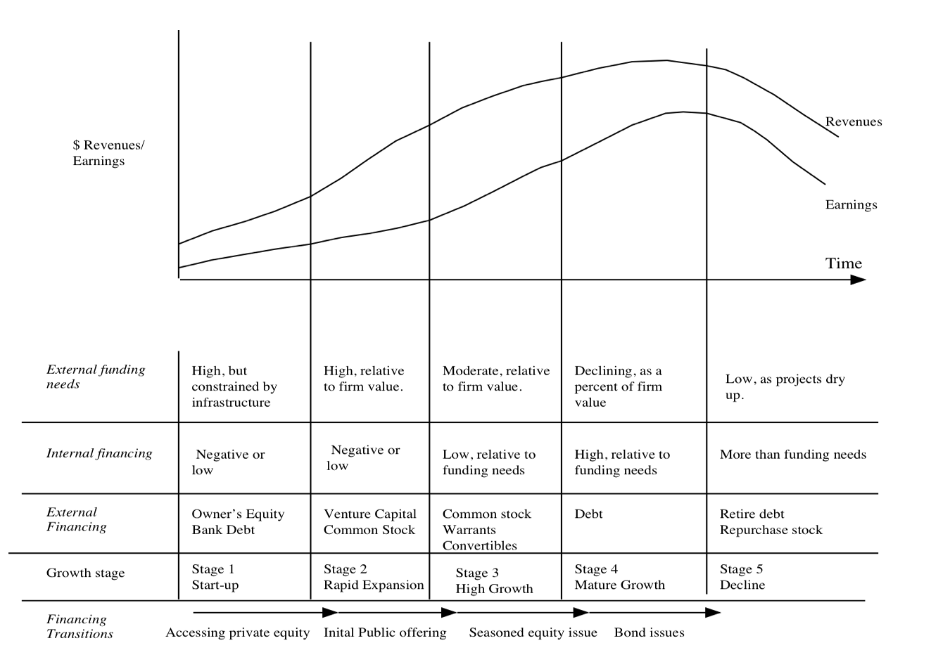
\includegraphics[width=0.35\textwidth]{./planning.png}
\hfill
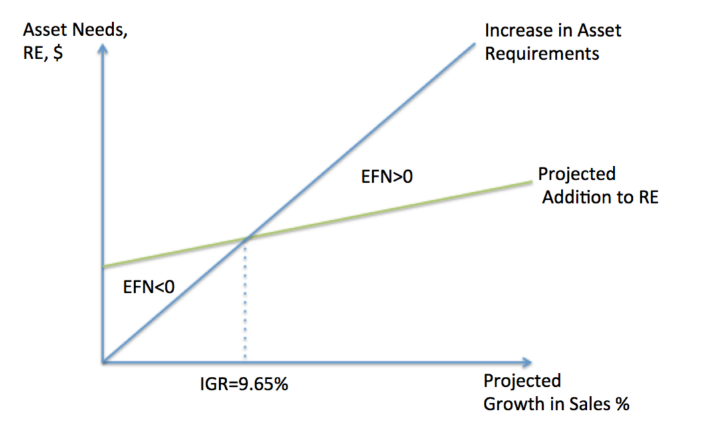
\includegraphics[width=0.35\textwidth]{./efn.png}
\end{document}
